\begin{frame}{Procedure between $t^n$ and $t^n + \Delta t^n=t^{n+1}$}
  \begin{footnotesize}
    \begin{overprint}
      %% Computation of matrices
      \onslide<1>
      \begin{equation*}
        \text{Discrete system: }\alert{M^L_{i}} \frac{\bar{\Ucb}^{i,n+1} - \bar{\Ucb}^{i,n}}{\Delta t^n}  - \alert{K_{ij}^\alpha} \bar{\Fcb}^{j,n}_{\alpha}  + \hat{\Fcb}^{i,n}=  \vect{0}
      \end{equation*}
      \begin{columns}
        \begin{column}{0.4\textwidth}
          \begin{itemize}
          \item[(1)] Computation of matrices $M_i^L$ and $K_{ij}^\alpha$
          \end{itemize}
        \end{column}
        \vrule{}
        \begin{column}{0.6\textwidth}
          \begin{block}{Computation of matrices $M_i^L$ and $K_{ij}^\alpha$}
            \begin{columns}
              \begin{column}{0.3\textwidth}
                \vskip 0.9pt
                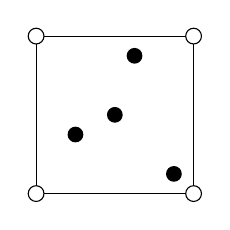
\begin{tikzpicture}
                  \draw (0,0) rectangle (2,2);
                  \fill[white] (0,0) circle (0.1); \fill[white] (0,2) circle (0.1); \fill[white] (2,0) circle (0.1); \fill[white] (2,2) circle (0.1);
                  \draw (0,0) circle (0.1); \draw (0,2) circle (0.1); \draw (2,0) circle (0.1); \draw (2,2) circle (0.1);
                  \fill[black] (0.5,0.75) circle (0.1); \fill[black] (1.25,1.75) circle (0.1); \fill[black] (1.75,0.25) circle (0.1); \fill[black] (1,1) circle (0.1);
                \end{tikzpicture}
              \end{column}
              \begin{column}{0.6\textwidth}
                States of particles known at time $t^n$:
                \begin{equation*}
                  \left\lbrace\begin{aligned}
                      & \vect{v}^{p,n},\tens{F}^{p,n},\tens{\Pi}^{p,n} \: \rightarrow \:\Ucb^{p,n},\Qcb^{p,n}\\
                      & \vect{X}^{p,n} \: \rightarrow \:M_i^{L,n},K_{ij}^{\alpha,n}
                    \end{aligned}\right.
                \end{equation*}
                
              \end{column}
            \end{columns}
          \end{block}
        \end{column}
      \end{columns}

      %% Particles -> Nodes
      \onslide<2>
      \begin{equation*}
        \text{Discrete system: }M^L_{i} \frac{\bar{\Ucb}^{i,n+1} - \alert{\bar{\Ucb}^{i,n}}}{\Delta t^n}  - K_{ij}^\alpha \bar{\Fcb}^{j,n}_{\alpha}  + \hat{\Fcb}^{i,n}=  \vect{0}
      \end{equation*}
      \begin{columns}
        \begin{column}{0.4\textwidth}
          \begin{itemize}
          \item[(1)] Computation of matrices $M_i^L$ and $K_{ij}^\alpha$
          \item[(2)] Projection particles $\rightarrow$ nodes
          \end{itemize}
        \end{column}
        \vrule{}
        \begin{column}{0.6\textwidth}
          \begin{block}{Projection particles $\rightarrow$ nodes}
            \begin{columns}
              \begin{column}{0.3\textwidth}
                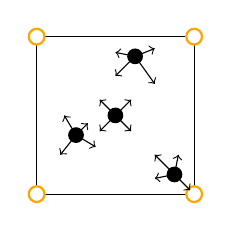
\begin{tikzpicture}
                  \draw (0,0) rectangle (2,2);
                  \fill[white] (0,0) circle (0.1); \fill[white] (0,2) circle (0.1); \fill[white] (2,0) circle (0.1); \fill[white] (2,2) circle (0.1);
                  \draw[Orange,thick] (0,0) circle (0.1); \draw[Orange,thick] (0,2) circle (0.1); \draw[Orange,thick] (2,0) circle (0.1); \draw[Orange,thick] (2,2) circle (0.1);
                  \fill[black] (0.5,0.75) circle (0.1); \fill[black] (1.25,1.75) circle (0.1); \fill[black] (1.75,0.25) circle (0.1); \fill[black] (1,1) circle (0.1);
                  %% North arrows
                  \draw[->,black] (1.25,1.75) -- (1.5,1.85);\draw[->,black] (1.25,1.75) -- (1.,1.8);\draw[->,black] (1.25,1.75) -- (1.,1.5);\draw[->,black] (1.25,1.75) -- (1.5,1.4);
                  %% West arrows
                  \draw[->,black] (0.5,0.75) -- (0.3,0.5);\draw[->,black] (0.5,0.75) -- (0.35,1.);\draw[->,black] (0.5,0.75) -- (0.75,.6);\draw[->,black] (0.5,0.75) -- (.65,0.9);
                  %% Center arrows
                  \draw[->,black] (1,1) -- (1.2,1.2);\draw[->,black] (1,1) -- (1.2,0.8);\draw[->,black] (1,1) -- (0.8,1.2);\draw[->,black] (1,1) -- (0.8,0.8);
                  %% South arrows
                  \draw[->,black] (1.75,0.25) -- (1.95,.05);\draw[->,black] (1.75,0.25) -- (1.8,.5);\draw[->,black] (1.75,0.25) -- (1.5,.5);\draw[->,black] (1.75,0.25) -- (1.5,0.2);
                \end{tikzpicture}
              \end{column}
              \begin{column}{0.6\textwidth}
                \begin{equation*}
                  \begin{aligned}
                    & M^{L,n}_i \alert{\bar{\Ucb}^{i,n}} = \sum_{p=1}^{N_p} m_p \bar{\Ucb}^{p,n}\\
                    & M^{L,n}_i \alert{\Qcb^{i,n}} = \sum_{p=1}^{N_p} m_p \Qcb^{p,n}
                  \end{aligned}
                \end{equation*}
              \end{column}
            \end{columns}
          \end{block}
        \end{column}
      \end{columns}
      
      %% Computation of numerical fluxes (volume + intercell)
      \onslide<3>
      \begin{equation*}
        \text{Discrete system: }M^L_{i} \frac{\bar{\Ucb}^{i,n+1} - \bar{\Ucb}^{i,n}}{\Delta t^n}  - K_{ij}^\alpha \alert{\bar{\Fcb}^{j,n}_{\alpha}}  + \alert{\hat{\Fcb}^{i,n}}=  \vect{0}
      \end{equation*}
      \begin{columns}
        \begin{column}{0.4\textwidth}
          \begin{itemize}
          \item[(1)] Computation of matrices $M_i^L$ and $K_{ij}^\alpha$
          \item[(2)] Projection particles $\rightarrow$ nodes
          \item[(3)] Computation of fluxes
          \end{itemize}
        \end{column}
        \vrule{}
        \begin{column}{0.6\textwidth}
          \begin{block}{Computation of fluxes}
            \begin{columns}
              \begin{column}{0.4\textwidth}
                \begin{block}{\footnotesize Volume fluxes}
                  $\bar{\Ucb}^{i,n},\Qcb^{i,n} \rightarrow \bar{\Fcb}^{i,n}_\alpha$
                \end{block}
              \end{column}
              \begin{column}{0.55\textwidth}
                \begin{block}{\footnotesize Intercell fluxes}
                  Approximate Riemann solver $\rightarrow \hat{\Fcb}^i$
                \end{block}
              \end{column}
            \end{columns}
          \end{block}
        \end{column}
      \end{columns}
      
      %% Time integration + Interpolation
      \onslide<4>
      \begin{equation*}
        \text{Discrete system: }M^L_{i} \frac{\alert{\bar{\Ucb}^{i,n+1}} - \bar{\Ucb}^{i,n}}{\Delta t^n}  - K_{ij}^\alpha \bar{\Fcb}^{j,n}_{\alpha}  + \hat{\Fcb}^{i,n}=  \vect{0}
      \end{equation*}
      \begin{columns}
        \begin{column}{0.4\textwidth}
          \begin{itemize}
          \item[(1)] Computation of matrices $M_i^L$ and $K_{ij}^\alpha$
          \item[(2)] Projection particles $\rightarrow$ nodes
          \item[(3)] Computation of fluxes
          \item[(4)] Explicit time integration; Interpolation
          \end{itemize}
        \end{column}
        \vrule{}
        \begin{column}{0.6\textwidth}
          \begin{block}{Explicit time integration; Interpolation}
            
            \begin{columns}
              \begin{column}{0.4\textwidth}
                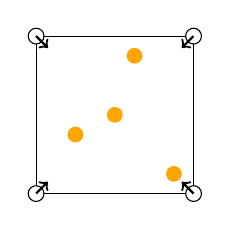
\begin{tikzpicture}
                  \draw (0,0) rectangle (2,2);
                  \fill[white] (0,0) circle (0.1); \fill[white] (0,2) circle (0.1); \fill[white] (2,0) circle (0.1); \fill[white] (2,2) circle (0.1);
                  \draw (0,0) circle (0.1); \draw (0,2) circle (0.1); \draw (2,0) circle (0.1); \draw (2,2) circle (0.1);
                  \draw[->,thick] (0,0) -- (0.15,0.15);
                  \draw[->,thick] (2,0) -- (1.85,0.15);
                  \draw[->,thick] (2,2) -- (1.85,1.85);
                  \draw[->,thick] (0,2) -- (.15,1.85);
                  
                  \fill[Orange] (0.5,0.75) circle (0.1); \fill[Orange] (1.25,1.75) circle (0.1); \fill[Orange] (1.75,0.25) circle (0.1); \fill[Orange] (1,1) circle (0.1);
                  
                  % \fill[black!50] (0.5,0.75) circle (0.1); \fill[black!50] (1.25,1.75) circle (0.1); \fill[black!50] (1.75,0.25) circle (0.1); \fill[black!50] (1,1) circle (0.1);
                  % \fill[black] (0.75,1.25) circle (0.1); \fill[black] (1.75,2.25) circle (0.1); \fill[black] (2.1,0.75) circle (0.1); \fill[black] (1.5,1.5) circle (0.1);
                  % \path[->,thick,black] (0.5,0.75) edge[bend left] (0.73,1.22);
                  % \path[->,thick,black] (1.25,1.75) edge[bend right] (1.75,2.21);
                  % \path[->,thick,black](1.75,0.25) edge[bend left] (2.,0.75);
                  % \path[->,thick,black](1,1) edge[bend right] (1.5,1.4);
                \end{tikzpicture}
              \end{column}
              \begin{column}{0.55\textwidth}
                \begin{equation*}
                  \alert{\bar{\Ucb}^{p,n+1}}=\sum_{i=1}^{N_{nodes}} S_{i}(\vect{X}^{p}) \bar{\Ucb}^{i,n+1}
                \end{equation*}
              \end{column}
            \end{columns}
          \end{block}
        \end{column}
      \end{columns}
           
      %% Kinematic and constitutive updates
      \onslide<5>
      \begin{columns}
        \begin{column}{0.4\textwidth}
          \begin{itemize}
          \item[(1)] Computation of matrices $M_i^L$ and $K_{ij}^\alpha$
          \item[(2)] Projection particles $\rightarrow$ nodes
          \item[(3)] Computation of fluxes
          \item[(4)] Explicit time integration; Interpolation
          \item[(5)] Kinematics and constitutive updates
          \end{itemize}
        \end{column}
        \vrule{}
        \begin{column}{0.6\textwidth}
          \begin{block}{Kinematics and constitutive updates}
            \begin{columns}
              \begin{column}{0.4\textwidth}
                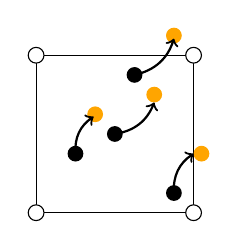
\begin{tikzpicture}
                  \draw (0,0) rectangle (2,2);
                  \fill[white] (0,0) circle (0.1); \fill[white] (0,2) circle (0.1); \fill[white] (2,0) circle (0.1); \fill[white] (2,2) circle (0.1);
                  \draw (0,0) circle (0.1); \draw (0,2) circle (0.1); \draw (2,0) circle (0.1); \draw (2,2) circle (0.1);
                  \fill[black] (0.5,0.75) circle (0.1); \fill[black] (1.25,1.75) circle (0.1); \fill[black] (1.75,0.25) circle (0.1); \fill[black] (1,1) circle (0.1);
                  \fill[Orange] (0.75,1.25) circle (0.1); \fill[Orange] (1.75,2.25) circle (0.1); \fill[Orange] (2.1,0.75) circle (0.1); \fill[Orange] (1.5,1.5) circle (0.1);
                  \path[->,thick,black] (0.5,0.75) edge[bend left] (0.73,1.22);
                  \path[->,thick,black] (1.25,1.75) edge[bend right] (1.75,2.21);
                  \path[->,thick,black](1.75,0.25) edge[bend left] (2.,0.75);
                  \path[->,thick,black](1,1) edge[bend right] (1.5,1.4);
                \end{tikzpicture}
              \end{column}
              \begin{column}{0.55\textwidth}
                \begin{flalign*}
                  \begin{aligned}
                    & \alert{\tens{\Pi}^{p,n+1}}=g(\tens{F}^{p,n+1})\\
                    & \alert{\vect{\varphi}^{p,n+1}}= \vect{\varphi}^{p,n} +\Delta t^n \vect{v}^{p,n+1}
                  \end{aligned}
                \end{flalign*}
              \end{column}
            \end{columns}
          \end{block}
        \end{column}
      \end{columns}
      
      
      %% Rebuild the grid if needed
      \onslide<6>
      \begin{columns}
        \begin{column}{0.4\textwidth}
          \begin{itemize}
          \item[(1)] Computation of matrices $M_i^L$ and $K_{ij}^\alpha$
          \item[(2)] Projection particles $\rightarrow$ nodes
          \item[(3)] Computation of fluxes
          \item[(4)] Explicit time integration; Interpolation
          \item[(5)] Kinematics and constitutive updates
          \item[(6)] Reconstruction of the grid (if needed) 
          \end{itemize}
        \end{column}
        \vrule{}
        \begin{column}{0.6\textwidth}
          \begin{block}{Reconstruction of the grid (if needed)}
            \begin{columns}
              \begin{column}{0.4\textwidth}
                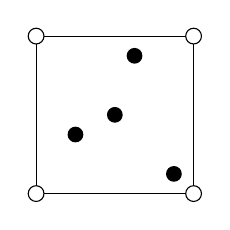
\begin{tikzpicture}
                  \draw (0,0) rectangle (2,2);
                  \fill[white] (0,0) circle (0.1); \fill[white] (0,2) circle (0.1); \fill[white] (2,0) circle (0.1); \fill[white] (2,2) circle (0.1);
                  \draw (0,0) circle (0.1); \draw (0,2) circle (0.1); \draw (2,0) circle (0.1); \draw (2,2) circle (0.1);
                  \fill[black] (0.5,0.75) circle (0.1); \fill[black] (1.25,1.75) circle (0.1); \fill[black] (1.75,0.25) circle (0.1); \fill[black] (1,1) circle (0.1);
                \end{tikzpicture}
              \end{column}
              \begin{column}{0.55\textwidth}
                \centering
                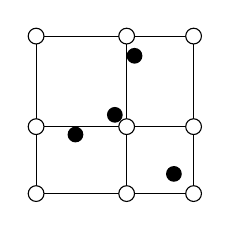
\begin{tikzpicture}
                  \draw (0,0) rectangle (2.,2.);
                  \draw (1.15,0.85) rectangle (2.,0);
                  \draw (1.15,0.85) rectangle (2.,2);
                  \draw (1.15,0.85) rectangle (0.,2);
                  %% Old nodes
                  \fill[white] (0,0) circle (0.1);
                  \fill[white] (0,2) circle (0.1);
                  \fill[white] (2,0) circle (0.1);
                  \fill[white] (2,2) circle (0.1);
                  \draw (0,0) circle (0.1);
                  \draw (0,2) circle (0.1);
                  \draw (2,0) circle (0.1);
                  \draw (2,2) circle (0.1);

                  %% Added nodes
                  \fill[white] (1.15,0.85) circle (0.1);
                  \fill[white] (0,0.85) circle (0.1);
                  \fill[white] (2,0.85) circle (0.1);
                  \fill[white] (1.15,0) circle (0.1);
                  \fill[white] (1.15,2) circle (0.1);
                  \draw (1.15,0.85) circle (0.1);
                  \draw (0,0.85) circle (0.1);
                  \draw (2,0.85) circle (0.1);
                  \draw (1.15,0) circle (0.1);
                  \draw (1.15,2) circle (0.1);

                  %% Particles
                  \fill[black] (0.5,0.75) circle (0.1); \fill[black] (1.25,1.75) circle (0.1); \fill[black] (1.75,0.25) circle (0.1); \fill[black] (1,1) circle (0.1);
                \end{tikzpicture}
              \end{column}
            \end{columns}
          \end{block}
        \end{column}
      \end{columns}
    \end{overprint}
  \end{footnotesize}
\end{frame}
